\chapter{Tecnologias Utilizadas}\label{tecnologias_utilizadas}

\section{Apache HTTP \textit{Server}}
O Apache HTTP \textit{Server} teve o seu primeiro lançamento publico em Abril de 1.995. Ele foi criado para ocupar o lugar deixado pelo HTTP \textit{Daemon}, na época o servidor para aplicações web mais utilizado no mundo. O HTTP \textit{Daemon} foi desenvolvido por Rob McCool quando ele trabalhava no \textit{National Center for Supercomputing Applications} – NCSA, na Universidade de Illinois, nos Estados Unidos. Porem, o desenvolvimento do HTTP \textit{Daemon} estagnou-se pois McCool havia saído da universidade. Como o código do HTTP \textit{Daemon} era aberto (\textit{open source}), vários desenvolvedores criaram correções e desenvolveram novas funcionalidades para o mesmo. Vendo a necessidade de juntar todos esses códigos desenvolvidos em separado, um grupo de desenvolvedores resolveram se juntar para compilar essas correções e novas funcionalidades. Usando como base a versão 1.3 do HTTP \textit{Daemon}, em Abril de 1.995 foi publicado o Apache HTTP \textit{Server} na versão 0.6.2. Também, nessa mesma época, foi criado o Apache \textit{Group}, grupo que mais tarde viria a se tornar o Apache \textit{Software Foundation}.\\
Hoje, quase 20 anos após o seu primeiro lançamento, o Apache HTTP \textit{Server} é o servidor HTTP mais utilizado no mundo e a sua versão estável atual é a 2.4.\\

\section{NGINX}
O NGINX (lê-se \textit{Engine-X}) foi criado pelo russo Igor Sysoev em 2.002 tendo a primeira versão publica sendo publicada em 2.004. O NGINX foi desenvolvido com o intuito de resolver o C10K \textit{problem}.\\
O C10k \textit{problem} consiste em solucionar o problema de atender a 10.000 requisições concorrentemente.\\
Diferentemente de outros servidores HTTP, o NGINX não usa \textit{threads} como base para manipular as requisições. Ao invés disso, ele utiliza uma arquitetura mais escalável orientada à eventos (\textit{event-driven}) assíncrona. Essa arquitetura utiliza uma quantidade pequena, porém previsível, de memória quando está trabalhando.\\

\begin{figure}
\centering
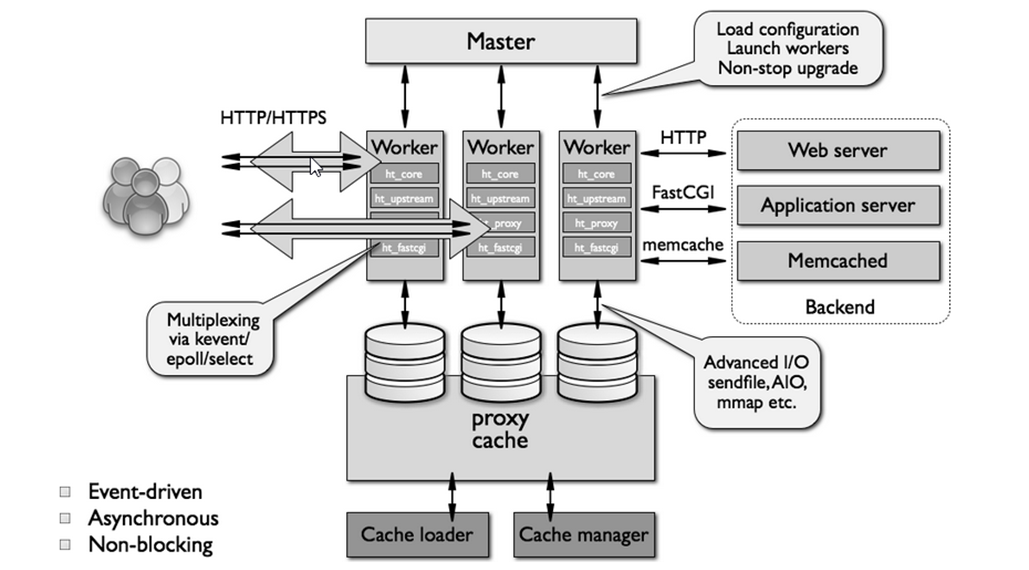
\includegraphics[scale=1]{figuras/nginx-how-it-works} 
\caption{Modelo de funcionamento do NGINX.}
\label{fig:nginx-comofunciona}
\end{figure}

O NGINX é utilizado por vários sítios de grande volume de tráfego como Netflix, GitHub, Pinterest, dentre outros.\\

\section{ApacheBench}
O ApacheBench foi criado em 1996 por Adam Twiss e, posteriormente doado ao Apache \textit{Group}. Originalmente, essa ferramenta foi desenvolvida para verificar o desempenho em servidores HTTP APACHE, mas hoje ela é utilizada para fazer testes de desempenho em  praticamente qualquer servidor HTTP.

\section{FastCGI}

\section{PHP}
\subsection{PHP-FPM}

\section{PostgreSQL}

\section{VirtualBox}

\section{Debian}

\section{APACHE HTTP \textit{Server versus} NGINX}
O APACHE, desde 1.995 tem sido o servidor HTTP mais utilizado no mundo. Em Outubro de 2.014, de acordo com pesquisa realizada em 1.028.932.208 de sítios pela empresa Netcraft, o APACHE era usado por 37,79\% (385.354.994) desses sítios, com o Microsoft IIS aparecendo em segundo com 33,58\% (345.485.419) e o NGINX em terceiro com 14,42\% (148.330.190) de participação nos sítios.\\

\begin{figure}
\centering
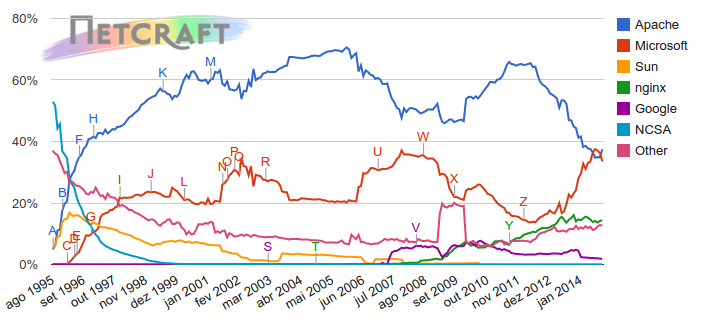
\includegraphics[scale=0.5]{figuras/grafico1}  
\caption{Utilização de Servidores \textit{web} no mundo.}
\label{fig:webservers-utilizacao}
\end{figure}

Nessa mesma pesquisa, entre os 1 milhão de sites mais acessados no mundo, o APACHE é utilizado em 50,19\% (501,922), com o NGINX em segundo lugar com 14,36\% (25,588,943).\\

\begin{figure}
\centering
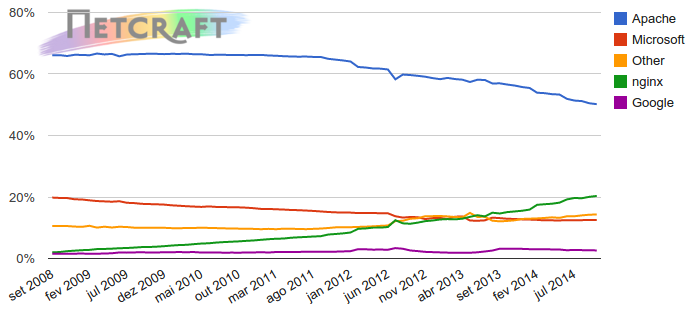
\includegraphics[scale=0.5]{figuras/grafico2} 
\caption{Utilização de Servidores \textit{web} entre os 1.000.000 de sítios mais acessados nomundo.}
\label{fig:webservers-utilizacao-milhao}
\end{figure}

Com a análise dos gráficos acima, é possível notar uma queda na utilização do APACHE em detrimento de outros servidores HTTP, sendo mais notório a queda na utilização entre os 1 milhão de sítios mais acessados. É possível notar também o aumento no uso do NGINX, principalmente entre os 1 milhão de sítios mais acessados no mundo.\\
Tendo sido desenvolvidos em épocas diferentes, o APACHE e o NGINX tem formas diferentes de servir as requisições que chegam no servidor.\\
De acordo com \cite{rowe}, o APACHE cria processos e \textit{threads} para lidar com as requisições. O administrador pode configurar o servidor para controlar o numero máximo de processos permitidos. Muitas \textit{threads} podem exaurir a memória principal(RAM) e pode forçar o servidor a usar memória \textit{SWAP}, degradando severamente o desempenho. Além disso, quando chega ao limite de processos, o APACHE passa a recusar conexões.